\documentclass[tikz,border=8pt]{standalone}

% Global stretch/compression factor for the entire diagram.
\newcommand{\stretchfactor}{1.0}

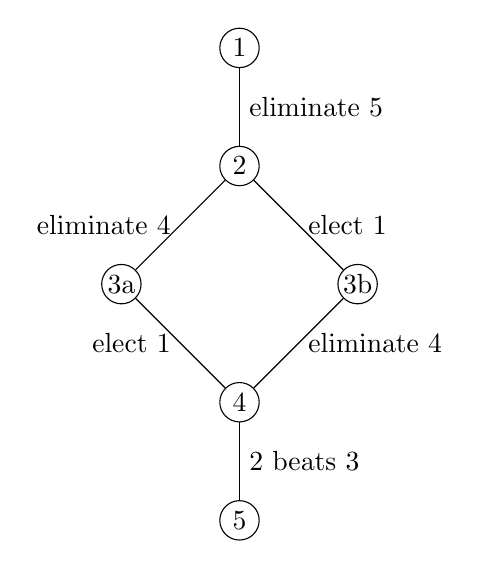
\begin{tikzpicture}[scale=1.5]
  \tikzstyle{graphnode}=[circle, draw, minimum size=0.5cm, inner sep=0pt]
  % Node definitions
  \node[graphnode] (n1) at (0,4) {1};
  \node[graphnode] (n2) at (0,3) {2};
  \node[graphnode] (n3) at (-1,2) {3a};
  \node[graphnode] (n4) at (1,2) {3b};
  \node[graphnode] (n5) at (0,1) {4};
  \node[graphnode] (n6) at (0,0) {5};

  % Edge definitions with placeholder labels
  \draw (n1) -- node[right]{eliminate 5} (n2);
  \draw (n2) -- node[left]{eliminate 4} (n3);
  \draw (n2) -- node[right]{elect 1} (n4);
  \draw (n3) -- node[left]{elect 1} (n5);
  \draw (n4) -- node[right]{eliminate 4} (n5);
  \draw (n5) -- node[right]{2 beats 3} (n6);
\end{tikzpicture}

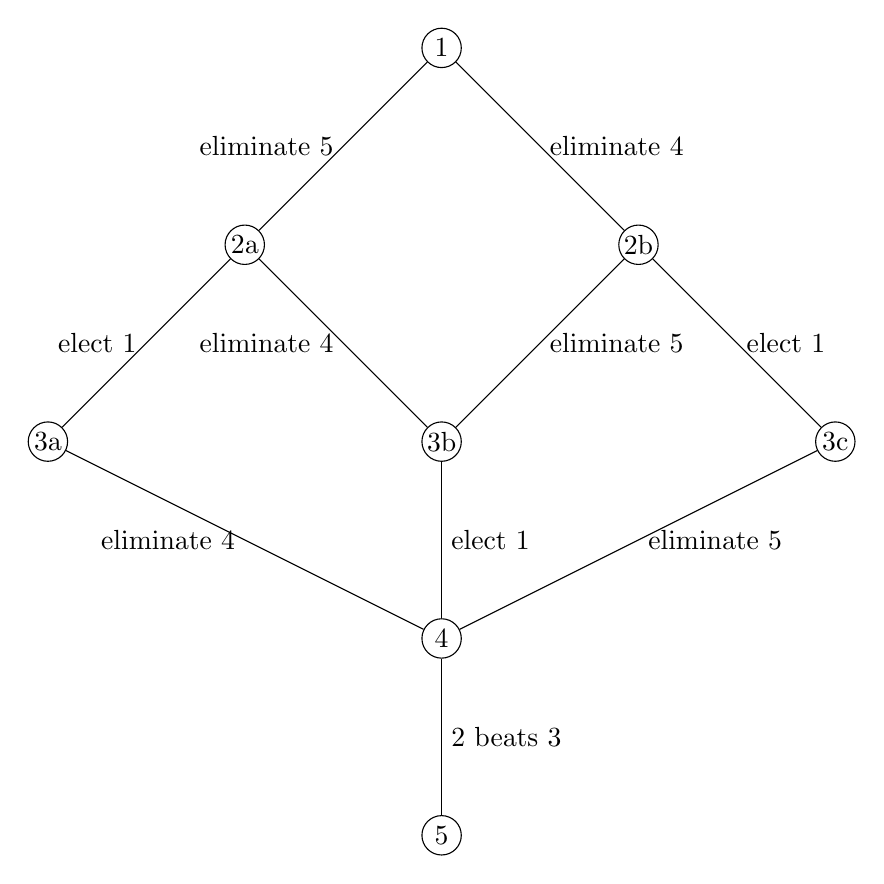
\begin{tikzpicture}[scale=2.5]
  \tikzstyle{graphnode}=[circle, draw, minimum size=0.5cm, inner sep=0pt]
  % Node definitions
  \node[graphnode] (n1) at (0,4) {1};
  \node[graphnode] (n2) at (-1,3) {2a};
  \node[graphnode] (n3) at (1,3) {2b};
  \node[graphnode] (n4) at (-2,2) {3a};
  \node[graphnode] (n5) at (0,2) {3b};
  \node[graphnode] (n6) at (2,2) {3c};
  \node[graphnode] (n7) at (0,1) {4};
  \node[graphnode] (n8) at (0,0) {5};

  % Edge definitions with placeholder labels
  \draw (n1) -- node[left]{eliminate 5} (n2);
  \draw (n1) -- node[right]{eliminate 4} (n3);
  \draw (n2) -- node[left]{elect 1} (n4);
  \draw (n2) -- node[left]{eliminate 4} (n5);
  \draw (n3) -- node[right]{eliminate 5} (n5);
  \draw (n3) -- node[right]{elect 1} (n6);
  \draw (n4) -- node[left]{eliminate 4} (n7);
  \draw (n5) -- node[right]{elect 1} (n7);
  \draw (n6) -- node[right]{eliminate 5} (n7);
  \draw (n7) -- node[right]{2 beats 3} (n8);
\end{tikzpicture}
